%!TEX TS-program = xelatex

% HSE Beamer Theme
% by Danil Fedorovykh
% http://hse.ru/staff/df
%
% Version 2.0 (English)
% January 2022

%%% Set up the free HSE Sans font
%%% https://www.hse.ru/info/brandbook/#font

\documentclass[aspectratio=169]{beamer}

\newbool{russian}
\booltrue{russian} % Uncomment if in Russian
\usepackage{HSE-theme/beamerthemeHSE} % Load HSE theme
\usepackage[no-math]{fontspec}      % fonts loading
\usepackage{caption}
\usepackage{subfigure}
\usepackage{subcaption}
\usepackage{hyperref}
\usepackage[dvipsnames]{xcolor}
\usepackage{ragged2e}
\captionsetup[figure]{labelformat=empty}
\captionsetup[subfigure]{labelformat=empty}
\renewcommand*{\thesubfigure}{(\arabic{subfigure})}
\setsansfont{HSE Sans}
%\graphicspath{{./images/}}
\graphicspath{{/home/llyy/Yandex.Disk/personal/knowledge/general/algorithms_course/repo/algorithms_course/3_sorting_recursion/lection/images}}


%%% Информация об авторе и выступлении
\title[Title]{Алгоритмы и структуры данных} 
\subtitle{Лекция 3. Рекурсия, сортировки (продолжение)}
\author[Author's name]{Илья Сергеевич Бычков\\ \smallskip \scriptsize \url{ibychkov@hse.ru}}
\institute{НИУ ВШЭ - Нижний Новгород}
\date{\today}


\begin{document}

\frame[plain]{\titlepage}

%%%%%%%%%%%%%%%%%%%%%%%%%%%%%%%%%%%%%%%%%%%%%%%%%%%%%%%%%%%%%%%%%%%%%%%%%%%%%%%%%%%%%%%%%%%%%%%%%%
\begin{frame}[c]
%\frametitle{A first slide}

\begin{center}
\Huge Лекция 3.

\Huge Рекурсия, сортировки (продолжение)
\end{center}

\end{frame}

%%%%%%%%%%%%%%%%%%%%%%%%%%%%%%%%%%%%%%%%%%%%%%%%%%%%%%%%%%%%%%%%%%%%%%%%%%%%%%%%%%%%%%%%%%%%%%%%%%
\begin{frame}
\frametitle{Рекурсия, сортировки (продолжение)}
\framesubtitle{План лекции}

\begin{enumerate}
  \setcounter{enumi}{-1}
  \item{План лекции}
  \item{\textcolor{blue}{Введение в рекурсию}}
  \item{Сортировка слиянием}
  \item{Быстрая сортировка}
  \item{Дополнения}
\end{enumerate}
\end{frame}



%%%%%%%%%%%%%%%%%%%%%%%%%%%%%%%%%%%%%%%%%%%%%%%%%%%%%%%%%%%%%%%%%%%%%%%%%%%%%%%%%%%%%%%%%%%%%%%%%%
\begin{frame}
\frametitle{Введение в рекурсию}
\framesubtitle{Рекурсия}
\justifying
\textcolor{red}{Рекурсия} — алгоритмическией механизм, представляющий один из способов \newline организации повторяющихся действий. Механизм решения задачи через сведение её к самой себе, но для более простого случая.\newline\newline
Отличительные особенности рекурсии:
\begin{itemize}
\item{Выполняет повторяющиеся действия для разных данных}
\item{Каждое новое выполнение/вызов решает более простую и меньшую по размерам задачу}
\item{Необходим четко определённый базовый случай, для которого ответ тривиален и известен}
\item{Необходим контроль за количеством выполняемых подзадач}
\end{itemize}
\end{frame}

%%%%%%%%%%%%%%%%%%%%%%%%%%%%%%%%%%%%%%%%%%%%%%%%%%%%%%%%%%%%%%%%%%%%%%%%%%%%%%%%%%%%%%%%%%%%%%%%%%
\begin{frame}
\frametitle{Введение в рекурсию}
\framesubtitle{Рекурсия}
\justifying
Рассмотрим простые задачи на рекурсию
\begin{itemize}
\item{Факториал/Последовательнось Фибоначчи}
\item{Вывести все числа из [1,n]}
\item{Палиндромы}
\item{Сумма цифр}
\end{itemize}
\end{frame}

%%%%%%%%%%%%%%%%%%%%%%%%%%%%%%%%%%%%%%%%%%%%%%%%%%%%%%%%%%%%%%%%%%%%%%%%%%%%%%%%%%%%%%%%%%%%%%%%%%
\begin{frame}
\frametitle{Рекурсия, сортировки (продолжение)}
\framesubtitle{План лекции}

\begin{enumerate}
  \setcounter{enumi}{-1}
  \item{План лекции}
  \item{Введение в рекурсию}
  \item{\textcolor{blue}{Сортировка слиянием}}
  \item{Быстрая сортировка}
  \item{Дополнения}
\end{enumerate}
\end{frame}



%%%%%%%%%%%%%%%%%%%%%%%%%%%%%%%%%%%%%%%%%%%%%%%%%%%%%%%%%%%%%%%%%%%%%%%%%%%%%%%%%%%%%%%%%%%%%%%%%%
\begin{frame}
\frametitle{Сортировка слиянием}
\framesubtitle{Общая информация}
\justifying
\textcolor{red}{Сортировка слиянием (Merge sort)}\newline\newline
В алгоритме используется распространенная алгоритмическая парадигма, известная как \textcolor{blue}{“разделяй и властвуй” (divide and conquer)}. \newline
\begin{itemize}
\item{\textcolor{blue}{Разделение}. Определяется правило, по которому задача разбивается на несколько подзадач, которые представляют собой меньшие экземпляры той же самой задачи.}
\item{\textcolor{blue}{Властвование}. Рекурсивно решаются подзадачи. Если они достаточно малы, они решаются как базовый случай.}
\item{\textcolor{blue}{Объединение}.Решения подзадач объединяются в решение исходной задачи}
\end{itemize}

\end{frame}

%%%%%%%%%%%%%%%%%%%%%%%%%%%%%%%%%%%%%%%%%%%%%%%%%%%%%%%%%%%%%%%%%%%%%%%%%%%%%%%%%%%%%%%%%%%%%%%%%%
\begin{frame}
\frametitle{Сортировка слиянием}
\framesubtitle{Общая информация}
\justifying
\textcolor{red}{Сортировка слиянием (Merge sort)}
\begin{figure}
    \captionsetup[subfigure]{labelformat=empty}
    \centering
    \subfigure[{ \scriptsize Сортировка слиянием, Источник - \href{https://en.wikipedia.org/wiki/Merge_sort}{Wiki}}]{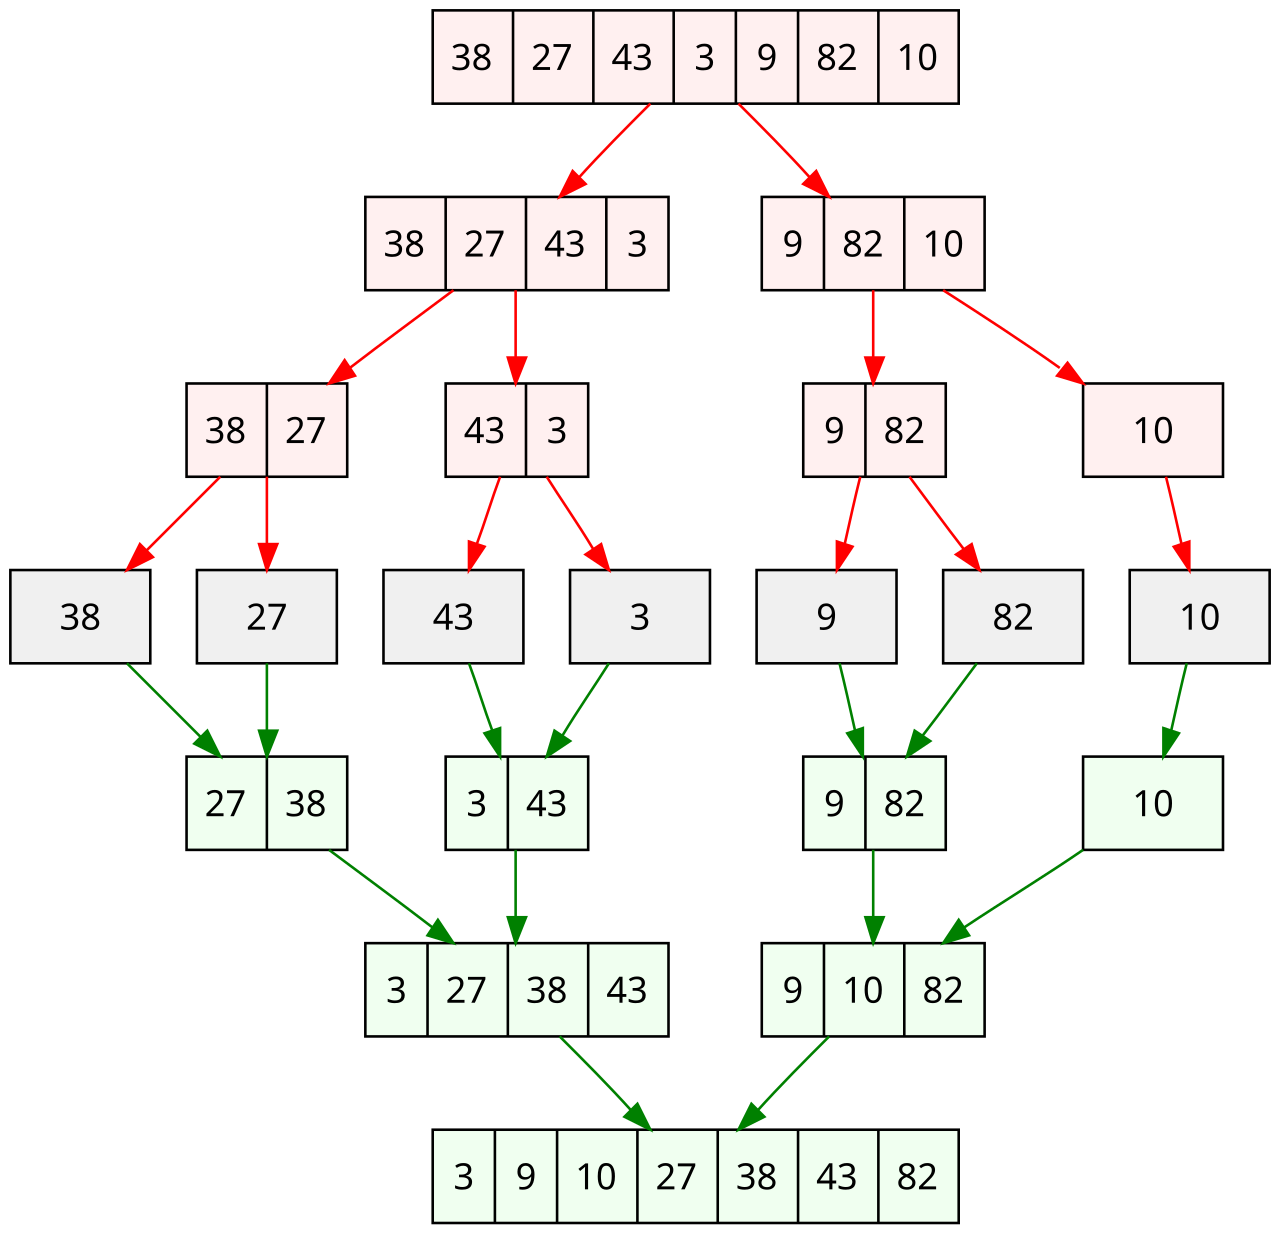
\includegraphics[width=70mm, height=58mm]{merge_example}} 
\end{figure}

\end{frame}

%%%%%%%%%%%%%%%%%%%%%%%%%%%%%%%%%%%%%%%%%%%%%%%%%%%%%%%%%%%%%%%%%%%%%%%%%%%%%%%%%%%%%%%%%%%%%%%%%%
\begin{frame}
\frametitle{Сортировка слиянием}
\framesubtitle{Основная функция}
\justifying
\textcolor{red}{Сортировка слиянием (Merge sort)}
\begin{figure}
    \captionsetup[subfigure]{labelformat=empty}
    \centering
    \subfigure[{ \scriptsize Сортировка слиянием - основная функция, Источник - \href{https://neerc.ifmo.ru/wiki/index.php?title=Сортировка_слиянием}{Neerc IFMO}}]{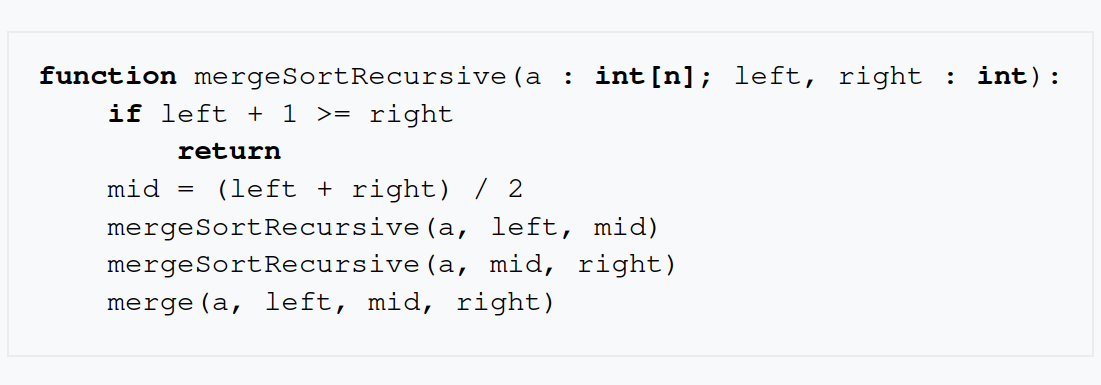
\includegraphics[width=140mm, height=52mm]{merge_recursive_main}} 
\end{figure}

\end{frame}


%%%%%%%%%%%%%%%%%%%%%%%%%%%%%%%%%%%%%%%%%%%%%%%%%%%%%%%%%%%%%%%%%%%%%%%%%%%%%%%%%%%%%%%%%%%%%%%%%%
\begin{frame}
\frametitle{Сортировка слиянием}
\framesubtitle{Процедура слияния}
\justifying
\textcolor{red}{Сортировка слиянием (Merge sort)}
\begin{figure}
    \captionsetup[subfigure]{labelformat=empty}
    \centering
    \subfigure[{ \scriptsize Сортировка слиянием - процедура слияния, Источник - \href{https://neerc.ifmo.ru/wiki/index.php?title=Сортировка_слиянием}{Neerc IFMO}}]{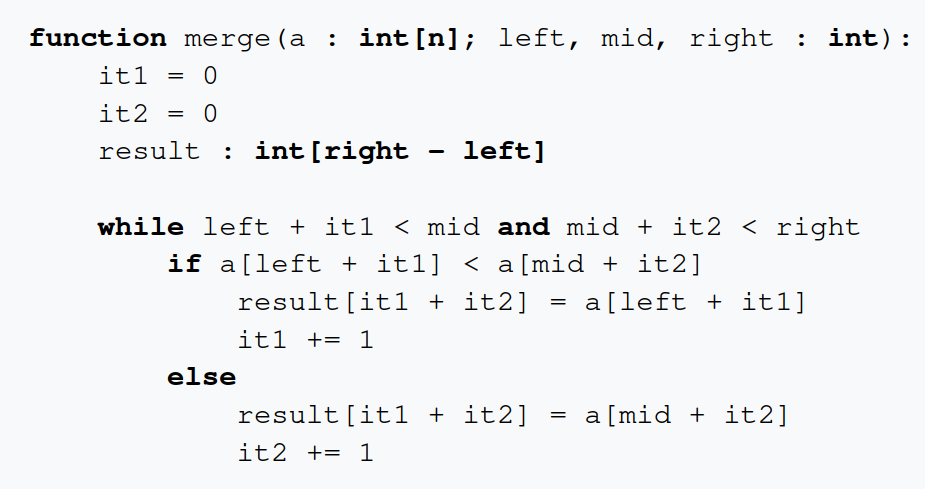
\includegraphics[width=100mm, height=52mm]{merge_merge_1}} 
\end{figure}

\end{frame}

%%%%%%%%%%%%%%%%%%%%%%%%%%%%%%%%%%%%%%%%%%%%%%%%%%%%%%%%%%%%%%%%%%%%%%%%%%%%%%%%%%%%%%%%%%%%%%%%%%
\begin{frame}
\frametitle{Сортировка слиянием}
\framesubtitle{Процедура слияния}
\justifying
\textcolor{red}{Сортировка слиянием (Merge sort)}
\begin{figure}
    \captionsetup[subfigure]{labelformat=empty}
    \centering
    \subfigure[{ \scriptsize Сортировка слиянием - процедура слияния, Источник - \href{https://neerc.ifmo.ru/wiki/index.php?title=Сортировка_слиянием}{Neerc IFMO}}]{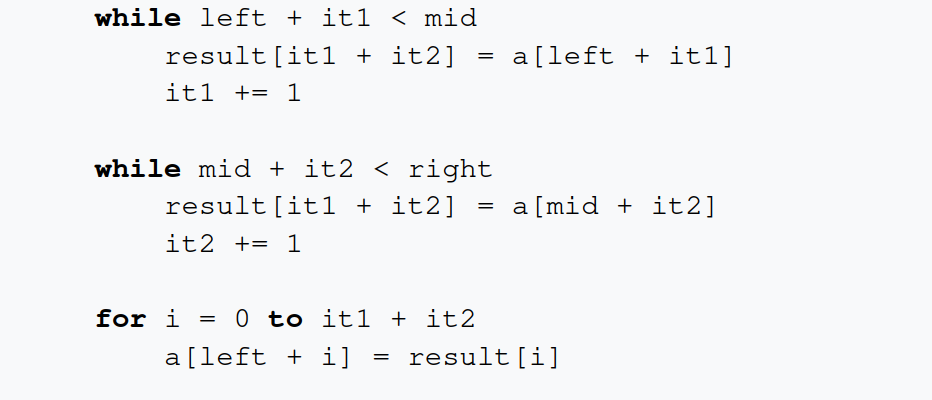
\includegraphics[width=120mm, height=52mm]{merge_merge_2}} 
\end{figure}

\end{frame}

%%%%%%%%%%%%%%%%%%%%%%%%%%%%%%%%%%%%%%%%%%%%%%%%%%%%%%%%%%%%%%%%%%%%%%%%%%%%%%%%%%%%%%%%%%%%%%%%%%
\begin{frame}
\frametitle{Сортировка слиянием}
\framesubtitle{Итеративная версия}
\justifying
\textcolor{red}{Сортировка слиянием (Merge sort)}\newline
Итеративная версия позволяет съэкономить примерно $\mathcal{O}(log_2 n)$ памяти
\begin{figure}
    \captionsetup[subfigure]{labelformat=empty}
    \centering
    \subfigure[{ \scriptsize Сортировка слиянием - итеративная версия, Источник - \href{https://neerc.ifmo.ru/wiki/index.php?title=Сортировка_слиянием}{Neerc IFMO}}]{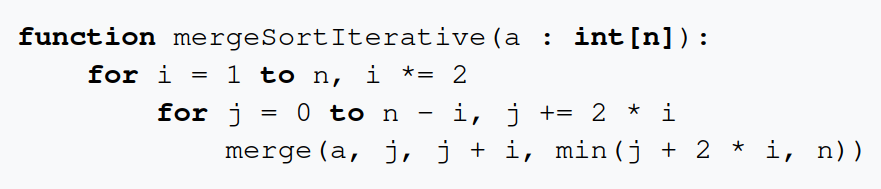
\includegraphics[width=120mm, height=30mm]{merge_iterative}} 
\end{figure}
\end{frame}

%%%%%%%%%%%%%%%%%%%%%%%%%%%%%%%%%%%%%%%%%%%%%%%%%%%%%%%%%%%%%%%%%%%%%%%%%%%%%%%%%%%%%%%%%%%%%%%%%%
\begin{frame}
\frametitle{Сортировка слиянием}
\framesubtitle{Сравнения}
\justifying
\begin{figure}
    \captionsetup[subfigure]{labelformat=empty}
    \centering
    \subfigure[{ \scriptsize Сортировка слиянием - сравнения, Источник - \href{https://algs4.cs.princeton.edu/lectures/keynote/22Mergesort.pdf}{Alg4cs Princeton - Sedgewick \& Wayne}}]{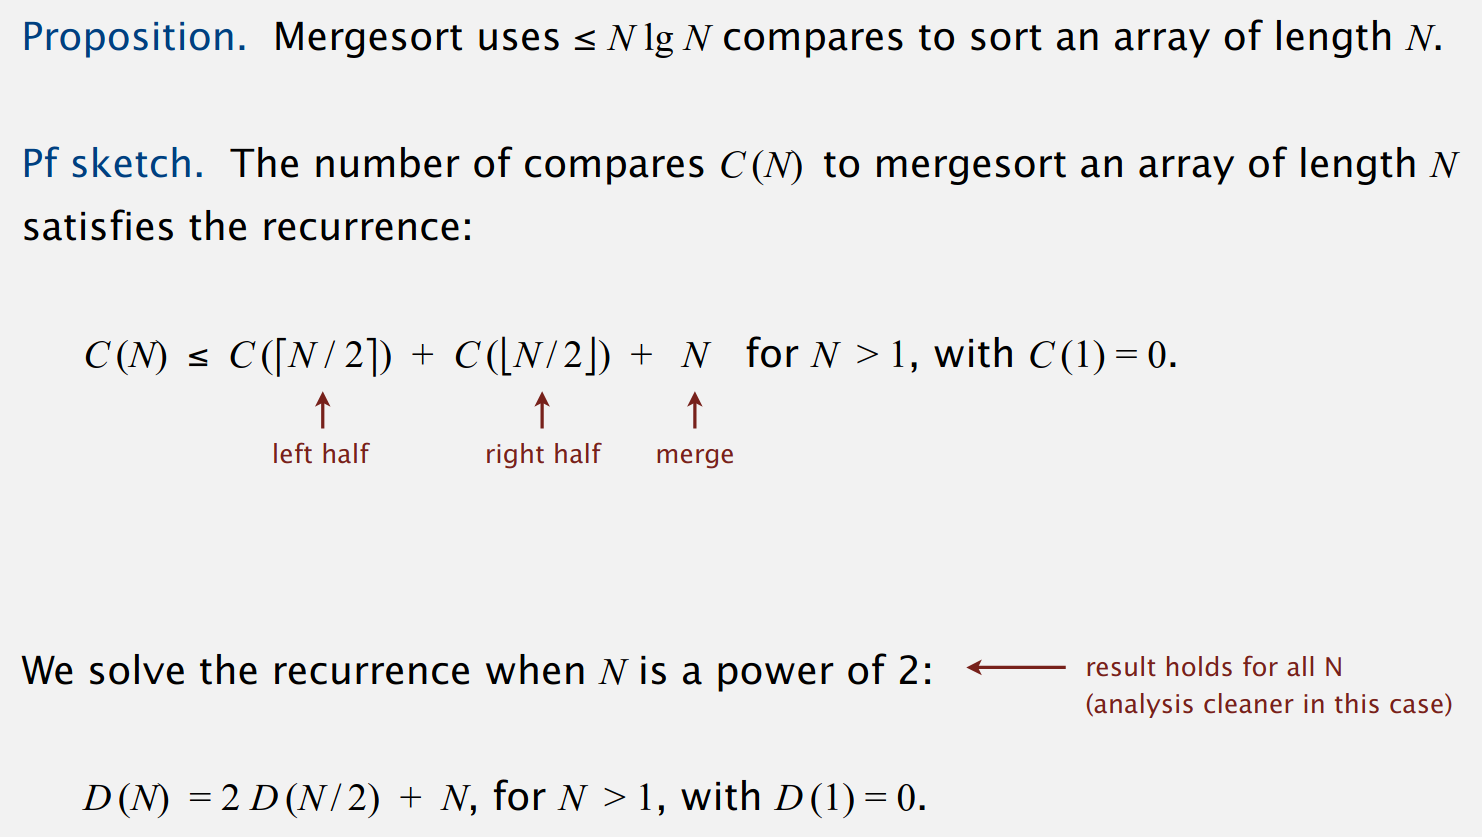
\includegraphics[width=130mm, height=65mm]{merge_compares_1}} 
\end{figure}
\end{frame}

%%%%%%%%%%%%%%%%%%%%%%%%%%%%%%%%%%%%%%%%%%%%%%%%%%%%%%%%%%%%%%%%%%%%%%%%%%%%%%%%%%%%%%%%%%%%%%%%%%
\begin{frame}
\frametitle{Сортировка слиянием}
\framesubtitle{Операции чтения/записи}
\justifying
\begin{figure}
    \captionsetup[subfigure]{labelformat=empty}
    \centering
    \subfigure[{ \scriptsize Сортировка слиянием - операции чтения, Источник - \href{https://algs4.cs.princeton.edu/lectures/keynote/22Mergesort.pdf}{Alg4cs Princeton - Sedgewick \& Wayne}}]{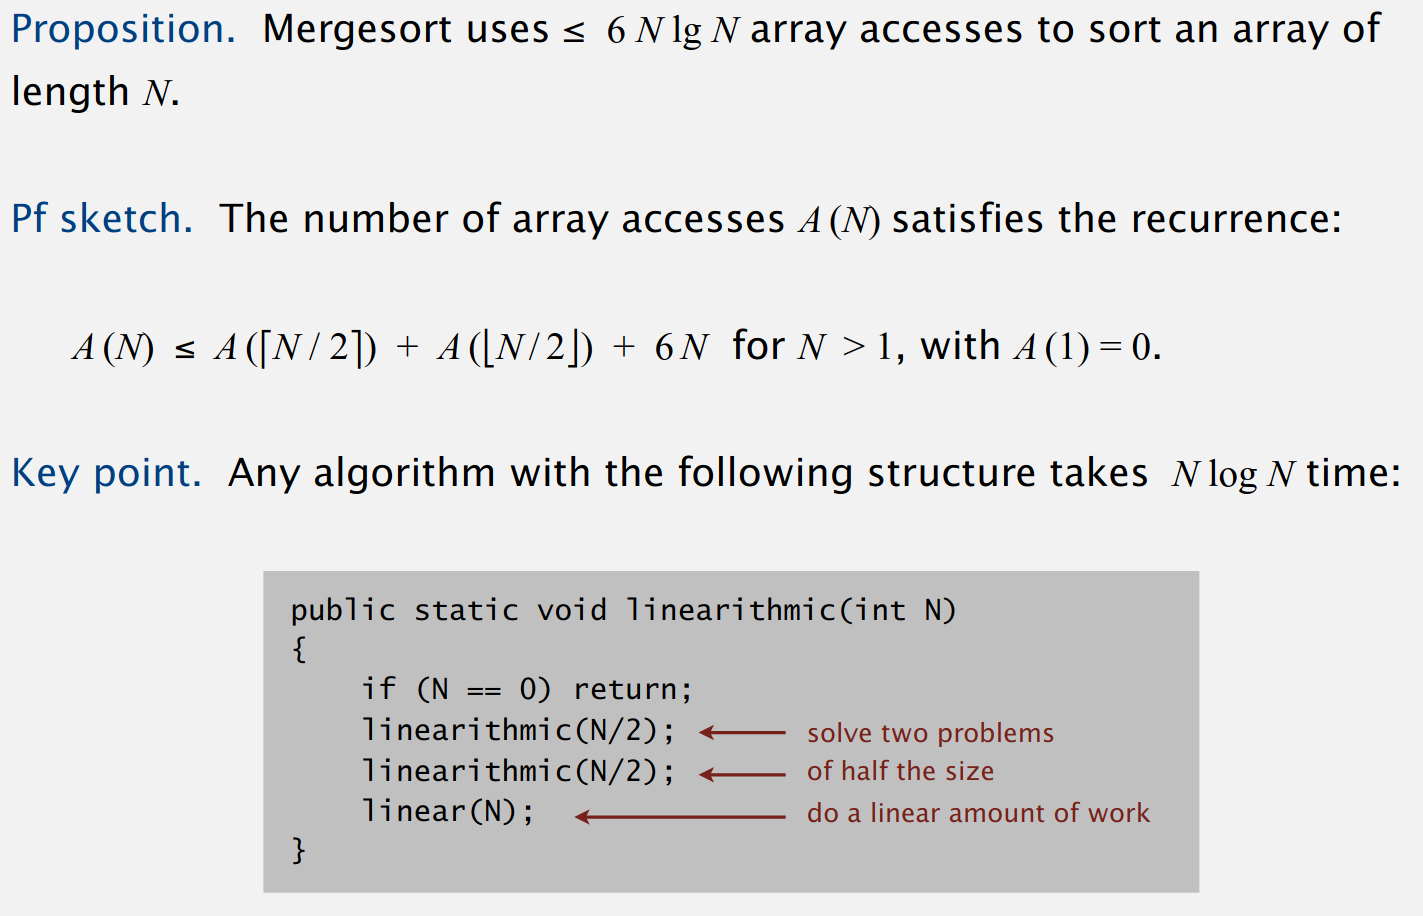
\includegraphics[width=125mm, height=65mm]{merge_accesses}} 
\end{figure}
\end{frame}

%%%%%%%%%%%%%%%%%%%%%%%%%%%%%%%%%%%%%%%%%%%%%%%%%%%%%%%%%%%%%%%%%%%%%%%%%%%%%%%%%%%%%%%%%%%%%%%%%%
\begin{frame}
\frametitle{Сортировка слиянием}
\framesubtitle{Улучшения}
\justifying
\begin{figure}
    \captionsetup[subfigure]{labelformat=empty}
    \centering
    \subfigure[{ \scriptsize Сортировка слиянием - улучшения, Источник - \href{https://algs4.cs.princeton.edu/lectures/keynote/22Mergesort.pdf}{Alg4cs Princeton - Sedgewick \& Wayne}}]{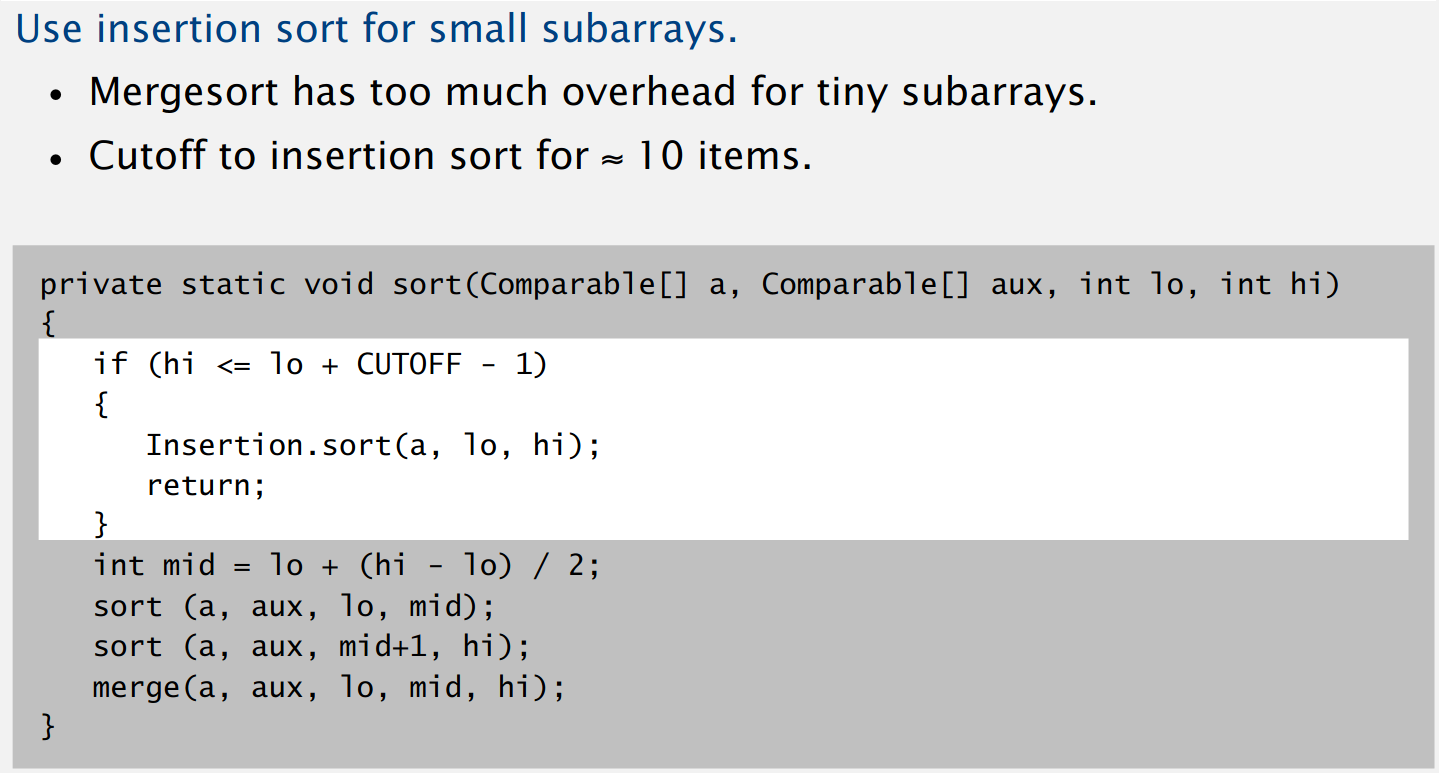
\includegraphics[width=125mm, height=65mm]{merge_insertion}} 
\end{figure}
\end{frame}

%%%%%%%%%%%%%%%%%%%%%%%%%%%%%%%%%%%%%%%%%%%%%%%%%%%%%%%%%%%%%%%%%%%%%%%%%%%%%%%%%%%%%%%%%%%%%%%%%%
\begin{frame}
\frametitle{Сортировка слиянием}
\framesubtitle{Улучшения}
\justifying
\begin{figure}
    \captionsetup[subfigure]{labelformat=empty}
    \centering
    \subfigure[{ \scriptsize Сортировка слиянием - улучшения, Источник - \href{https://algs4.cs.princeton.edu/lectures/keynote/22Mergesort.pdf}{Alg4cs Princeton - Sedgewick \& Wayne}}]{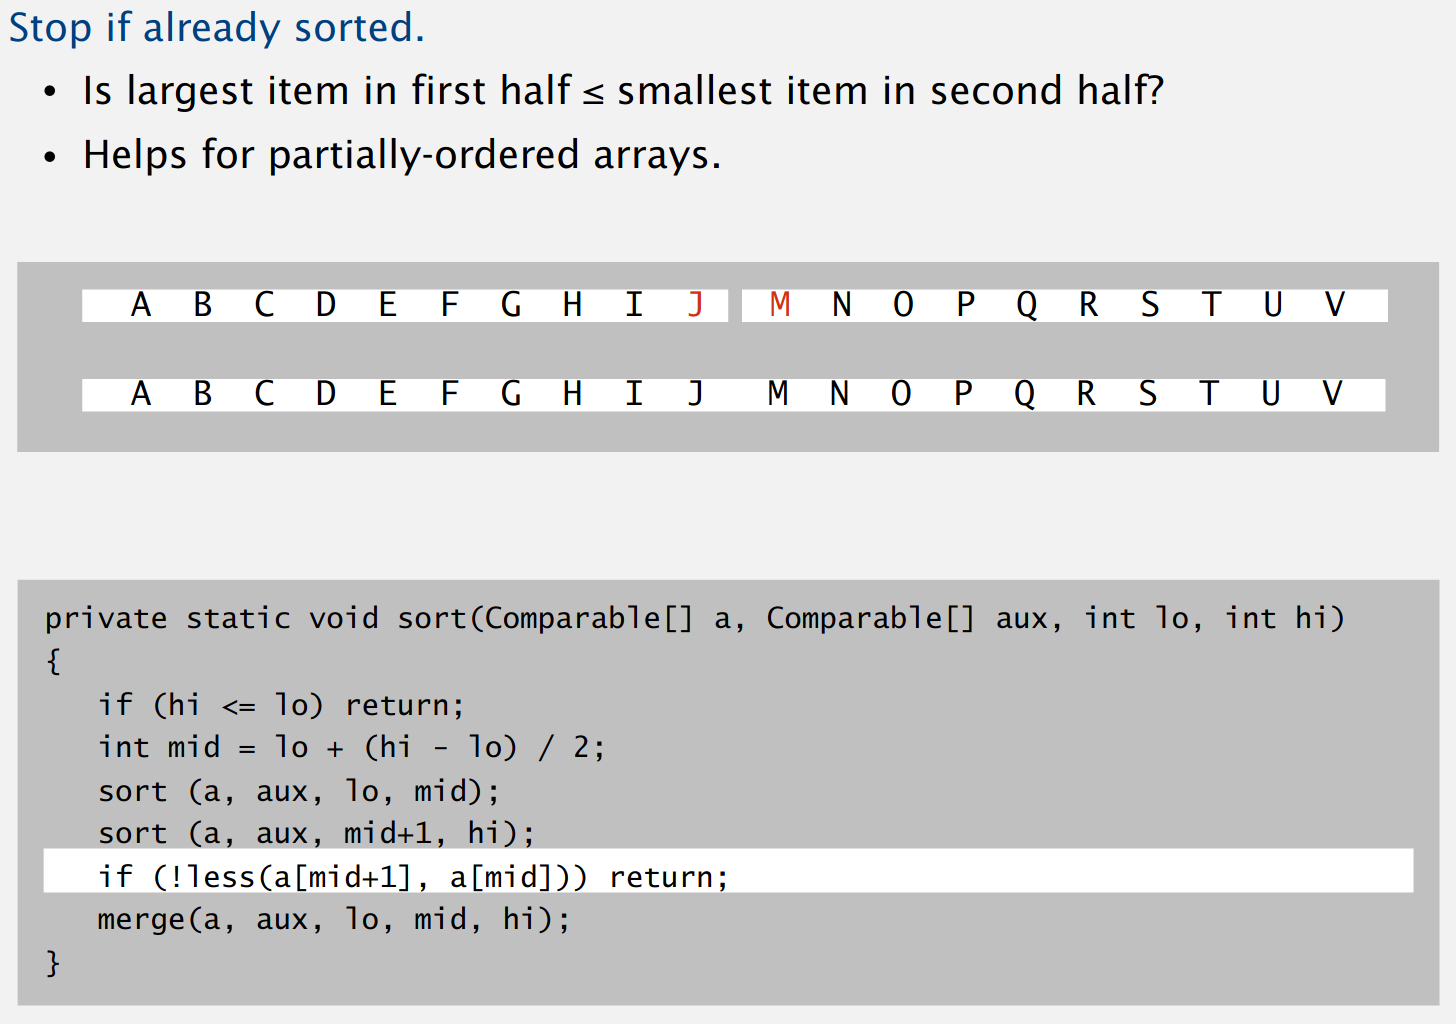
\includegraphics[width=115mm, height=65mm]{merge_already_sorted}} 
\end{figure}
\end{frame}

%%%%%%%%%%%%%%%%%%%%%%%%%%%%%%%%%%%%%%%%%%%%%%%%%%%%%%%%%%%%%%%%%%%%%%%%%%%%%%%%%%%%%%%%%%%%%%%%%%
\begin{frame}
\frametitle{Простые сортировки}
\framesubtitle{План лекции}

\begin{enumerate}
  \setcounter{enumi}{-1}
  \item{План лекции}
  \item{Введение в рекурсию}
  \item{Сортировка слиянием}
  \item{\textcolor{blue}{Быстрая сортировка}}
  \item{Дополнения}
\end{enumerate}
\end{frame}

%%%%%%%%%%%%%%%%%%%%%%%%%%%%%%%%%%%%%%%%%%%%%%%%%%%%%%%%%%%%%%%%%%%%%%%%%%%%%%%%%%%%%%%%%%%%%%%%%%
\begin{frame}
\frametitle{Быстрая сортировка}
\framesubtitle{Общая информация}
\justifying
\textcolor{red}{Быстрая сортировка (Quick sort)}\newline\newline
В алгоритме также используется парадигма “разделяй и властвуй”.\newline

Общая схема:

\begin{itemize}
\item{Из массива выбирается некоторый \textcolor{red}{опорный элемент (pivot)} a[i] }
\item{Запускается процедура разделения массива, которая перемещает все значения, меньшие, либо равные a[i], влево от него, а все значения, большие, либо равные a[i] – вправо}
\item{Рекурсивно запускаем процедуру для левой и правой частей}
\end{itemize}

\end{frame}

%%%%%%%%%%%%%%%%%%%%%%%%%%%%%%%%%%%%%%%%%%%%%%%%%%%%%%%%%%%%%%%%%%%%%%%%%%%%%%%%%%%%%%%%%%%%%%%%%%
\begin{frame}
\frametitle{Быстрая сортировка}
\framesubtitle{Пример}
\justifying
\textcolor{red}{Быстрая сортировка (Quick Sort)}
\begin{figure}
    \captionsetup[subfigure]{labelformat=empty}
    \centering
    \subfigure[{ \scriptsize Быстрая сортировка, Источник - \href{-}{Cormen et al., 3rd edition}}]{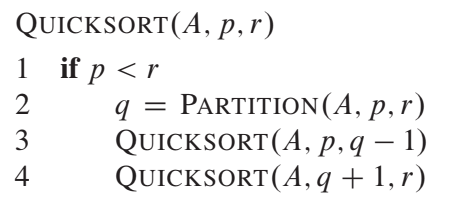
\includegraphics[width=60mm, height=25mm]{qs_main_pseudo}}
    \subfigure[{ \scriptsize Разбиение, Источник - \href{-}{Cormen et al., 3rd edition}}]{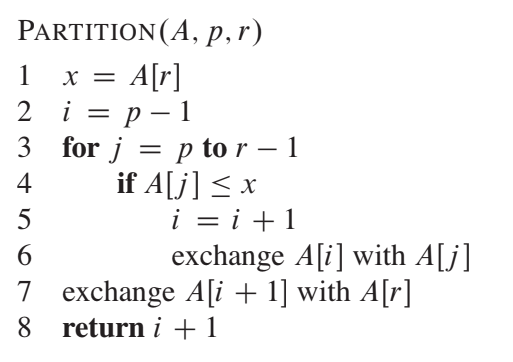
\includegraphics[width=75mm, height=50mm]{qs_lomuto_pseudo}} 
\end{figure}

\end{frame}

%%%%%%%%%%%%%%%%%%%%%%%%%%%%%%%%%%%%%%%%%%%%%%%%%%%%%%%%%%%%%%%%%%%%%%%%%%%%%%%%%%%%%%%%%%%%%%%%%%
\begin{frame}
\frametitle{Быстрая сортировка}
\framesubtitle{Пример}
\justifying
\textcolor{red}{Быстрая сортировка (Quick Sort)}
\begin{figure}
    \captionsetup[subfigure]{labelformat=empty}
    \centering
    \subfigure[{ \scriptsize Быстрая сортировка, Источник - \href{-}{Неизвестен}}]{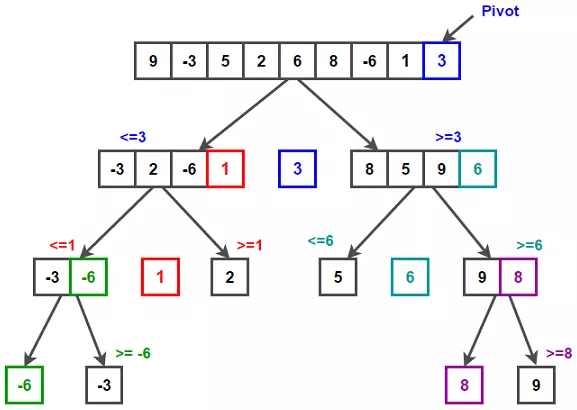
\includegraphics[width=90mm, height=59mm]{qs_example}} 
\end{figure}

\end{frame}

\begin{frame}
\frametitle{Быстрая сортировка}
\framesubtitle{Разбиение Ломуто}
\justifying
\textcolor{red}{Разбиение Ломуто (Lomuto Partition)}
\begin{figure}
    \captionsetup[subfigure]{labelformat=empty}
    \centering
    \subfigure[{ \scriptsize Разбиение Ломуто, Источник - \href{https://www.geeksforgeeks.org/hoares-vs-lomuto-partition-scheme-quicksort/}{Geeks4Geeks}}]{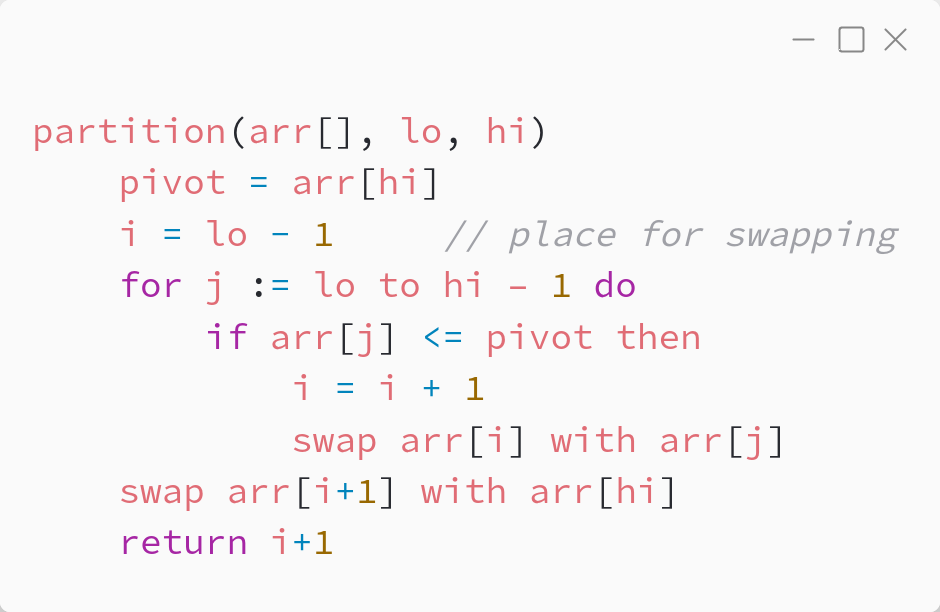
\includegraphics[width=100mm, height=59mm]{qs_lomuto}} 
\end{figure}
\end{frame}

\begin{frame}
\frametitle{Быстрая сортировка}
\framesubtitle{Разбиение Хоара}
\justifying
\begin{figure}
    \captionsetup[subfigure]{labelformat=empty}
    \centering
    \subfigure[{ \scriptsize Разбиение Хоара,  Источник - \href{https://www.geeksforgeeks.org/hoares-vs-lomuto-partition-scheme-quicksort/}{Geeks4Geeks}}]{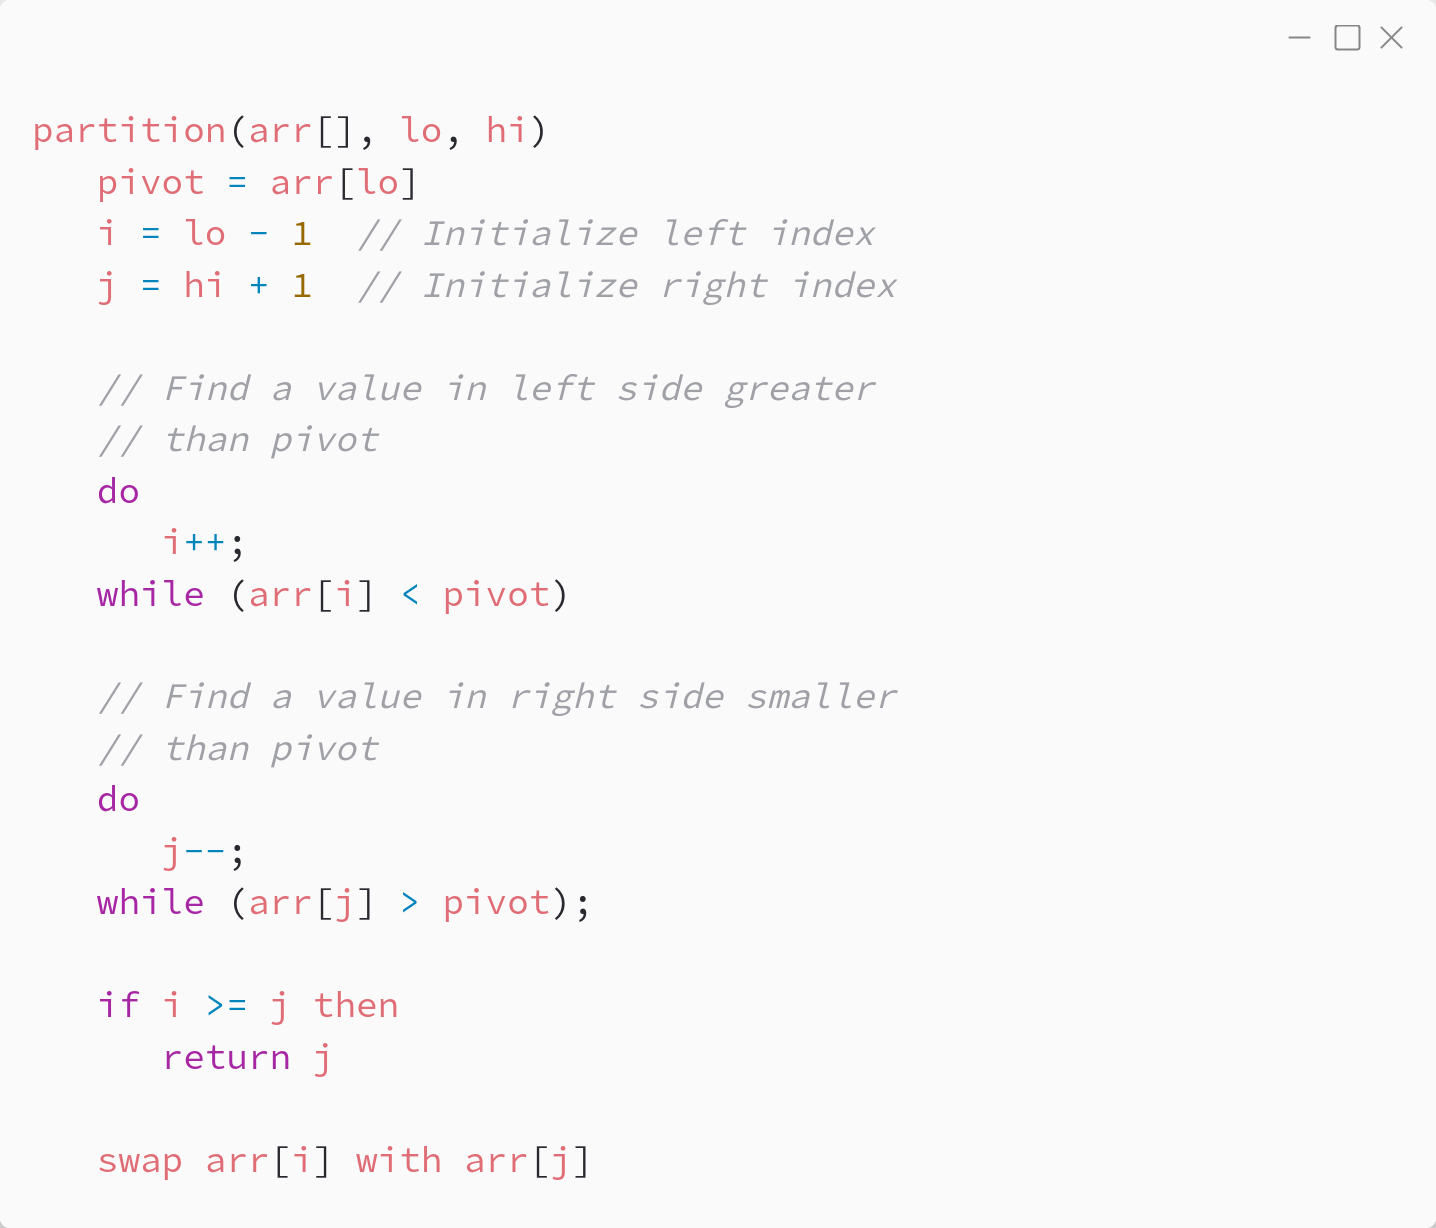
\includegraphics[width=83mm, height=64mm]{qs_hoare}} 
\end{figure}

\end{frame}

\begin{frame}
\frametitle{Быстрая сортировка}
\framesubtitle{Сложность}
\justifying
\begin{figure}
    \captionsetup[subfigure]{labelformat=empty}
    \centering
    \subfigure[{ \scriptsize Быстрая сортировка - Сложность, Источник - \href{https://algs4.cs.princeton.edu/lectures/keynote/22Mergesort.pdf}{Alg4cs Princeton - Sedgewick \& Wayne}}]{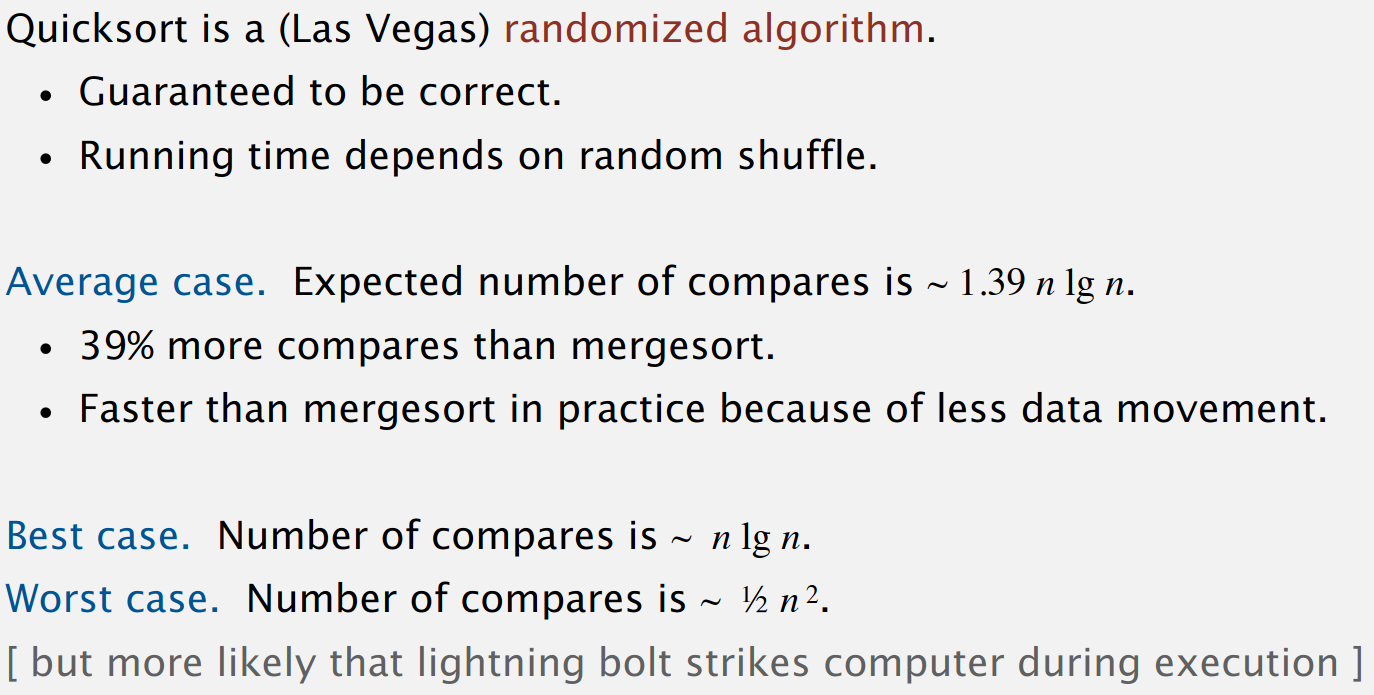
\includegraphics[width=120mm, height=60mm]{qs_complexity_cases}} 
\end{figure}

\end{frame}

%%%%%%%%%%%%%%%%%%%%%%%%%%%%%%%%%%%%%%%%%%%%%%%%%%%%%%%%%%%%%%%%%%%%%%%%%%%%%%%%%%%%%%%%%%%%%%%%%%
\begin{frame}
\frametitle{Порядковые статистики}
\framesubtitle{k-я порядковая статистика}
\justifying
\begin{figure}
    \captionsetup[subfigure]{labelformat=empty}
    \centering
    \subfigure[{ \scriptsize  k-я порядковая статистика, Источник - \href{https://algs4.cs.princeton.edu/lectures/keynote/22Mergesort.pdf}{Alg4cs Princeton - Sedgewick \& Wayne}}]{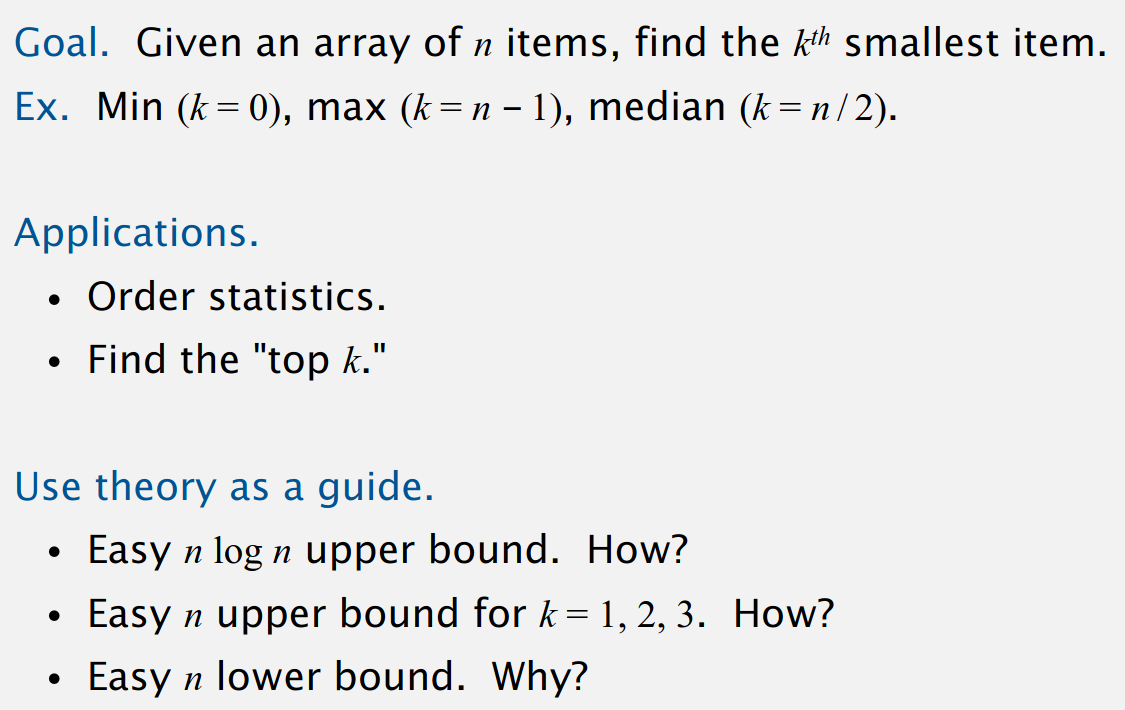
\includegraphics[width=100mm, height=60mm]{qselect}} 
\end{figure}
\end{frame}


%%%%%%%%%%%%%%%%%%%%%%%%%%%%%%%%%%%%%%%%%%%%%%%%%%%%%%%%%%%%%%%%%%%%%%%%%%%%%%%%%%%%%%%%%%%%%%%%%%
\begin{frame}
\frametitle{Порядковые статистики}
\framesubtitle{Quick-select}
\justifying
\begin{figure}
    \captionsetup[subfigure]{labelformat=empty}
    \centering
    \subfigure[{ \scriptsize  Разбиение, Источник - \href{https://algs4.cs.princeton.edu/lectures/keynote/22Mergesort.pdf}{Alg4cs Princeton - Sedgewick \& Wayne}}]{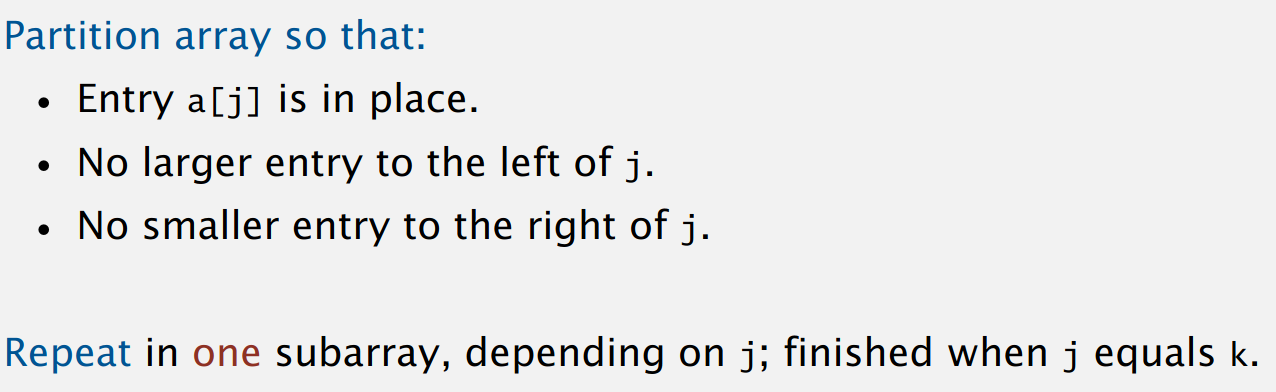
\includegraphics[width=75mm, height=25mm]{qs_common}} 
    \subfigure[{ \scriptsize  Quick-select, Источник - \href{https://algs4.cs.princeton.edu/lectures/keynote/22Mergesort.pdf}{Alg4cs Princeton - Sedgewick \& Wayne}}]{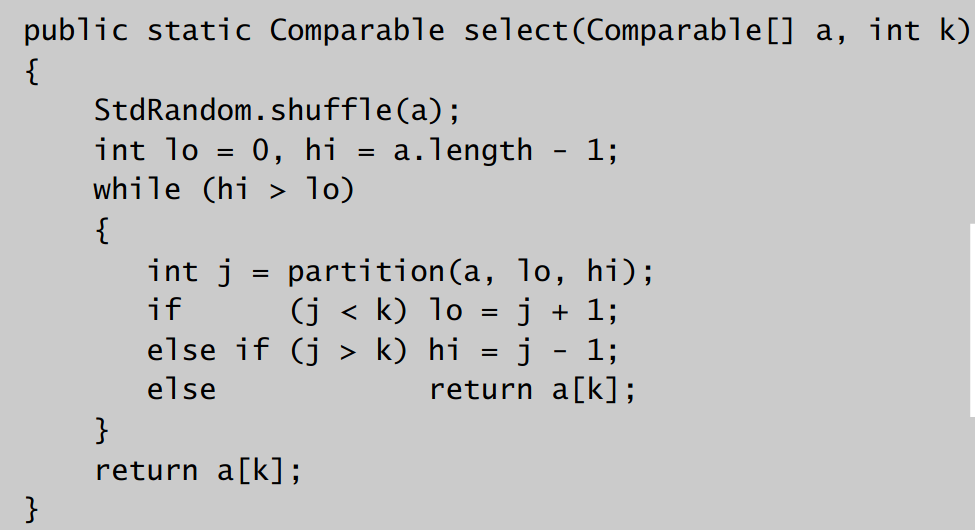
\includegraphics[width=60mm, height=40mm]{qs_pseudo}} 
\end{figure}
\end{frame}


%%%%%%%%%%%%%%%%%%%%%%%%%%%%%%%%%%%%%%%%%%%%%%%%%%%%%%%%%%%%%%%%%%%%%%%%%%%%%%%%%%%%%%%%%%%%%%%%%%
\begin{frame}
\frametitle{Простые сортировки}
\framesubtitle{План лекции}

\begin{enumerate}
  \setcounter{enumi}{-1}
  \item{План лекции}
  \item{Введение в рекурсию}
  \item{Сортировка слиянием}
  \item{Быстрая сортировка}
  \item{\textcolor{blue}{Дополнения}}
\end{enumerate}
\end{frame}

%%%%%%%%%%%%%%%%%%%%%%%%%%%%%%%%%%%%%%%%%%%%%%%%%%%%%%%%%%%%%%%%%%%%%%%%%%%%%%%%%%%%%%%%%%%%%%%%%%
\begin{frame}
\frametitle{Дополнения}
\framesubtitle{Сортировки на сравнениях}
\justifying
\begin{figure}
    \captionsetup[subfigure]{labelformat=empty}
    \centering
    \subfigure[{ \scriptsize  Сортировки на сравнениях, Источник - \href{https://algs4.cs.princeton.edu/lectures/keynote/22Mergesort.pdf}{Alg4cs Princeton - Sedgewick \& Wayne}}]{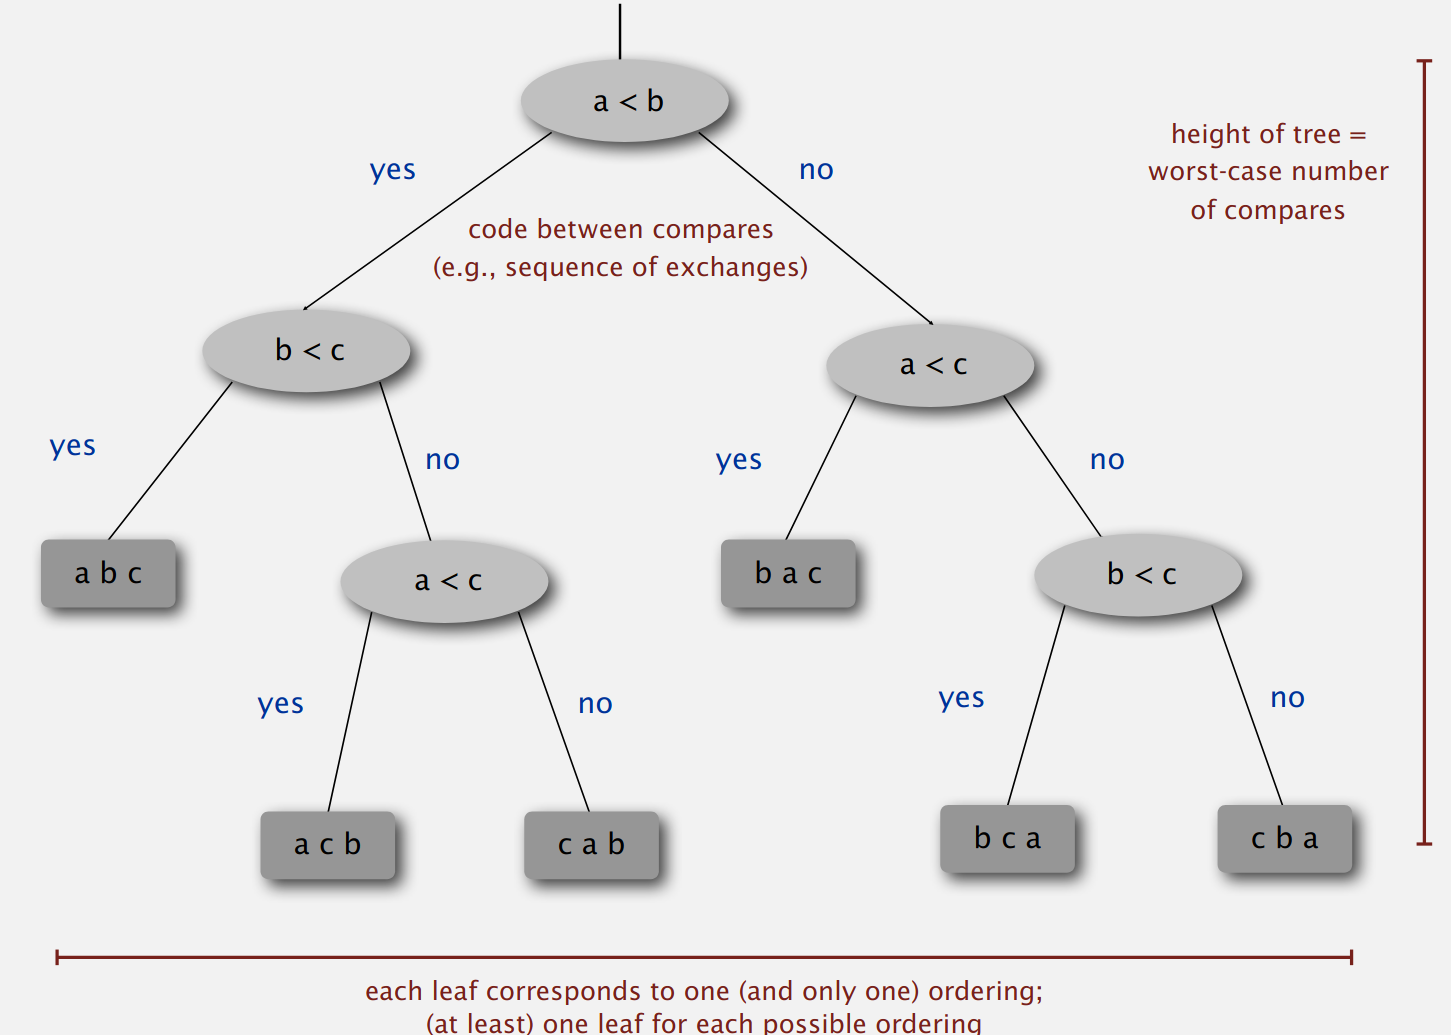
\includegraphics[width=120mm, height=65mm]{compare_based_tree}} 

\end{figure}
\end{frame}

%%%%%%%%%%%%%%%%%%%%%%%%%%%%%%%%%%%%%%%%%%%%%%%%%%%%%%%%%%%%%%%%%%%%%%%%%%%%%%%%%%%%%%%%%%%%%%%%%%
\begin{frame}
\frametitle{Дополнения}
\framesubtitle{Сортировки на сравнениях}
\justifying
\begin{figure}
    \captionsetup[subfigure]{labelformat=empty}
    \centering
    \subfigure[{ \scriptsize  Сортировки на сравнениях, Источник - \href{https://algs4.cs.princeton.edu/lectures/keynote/22Mergesort.pdf}{Alg4cs Princeton - Sedgewick \& Wayne}}]{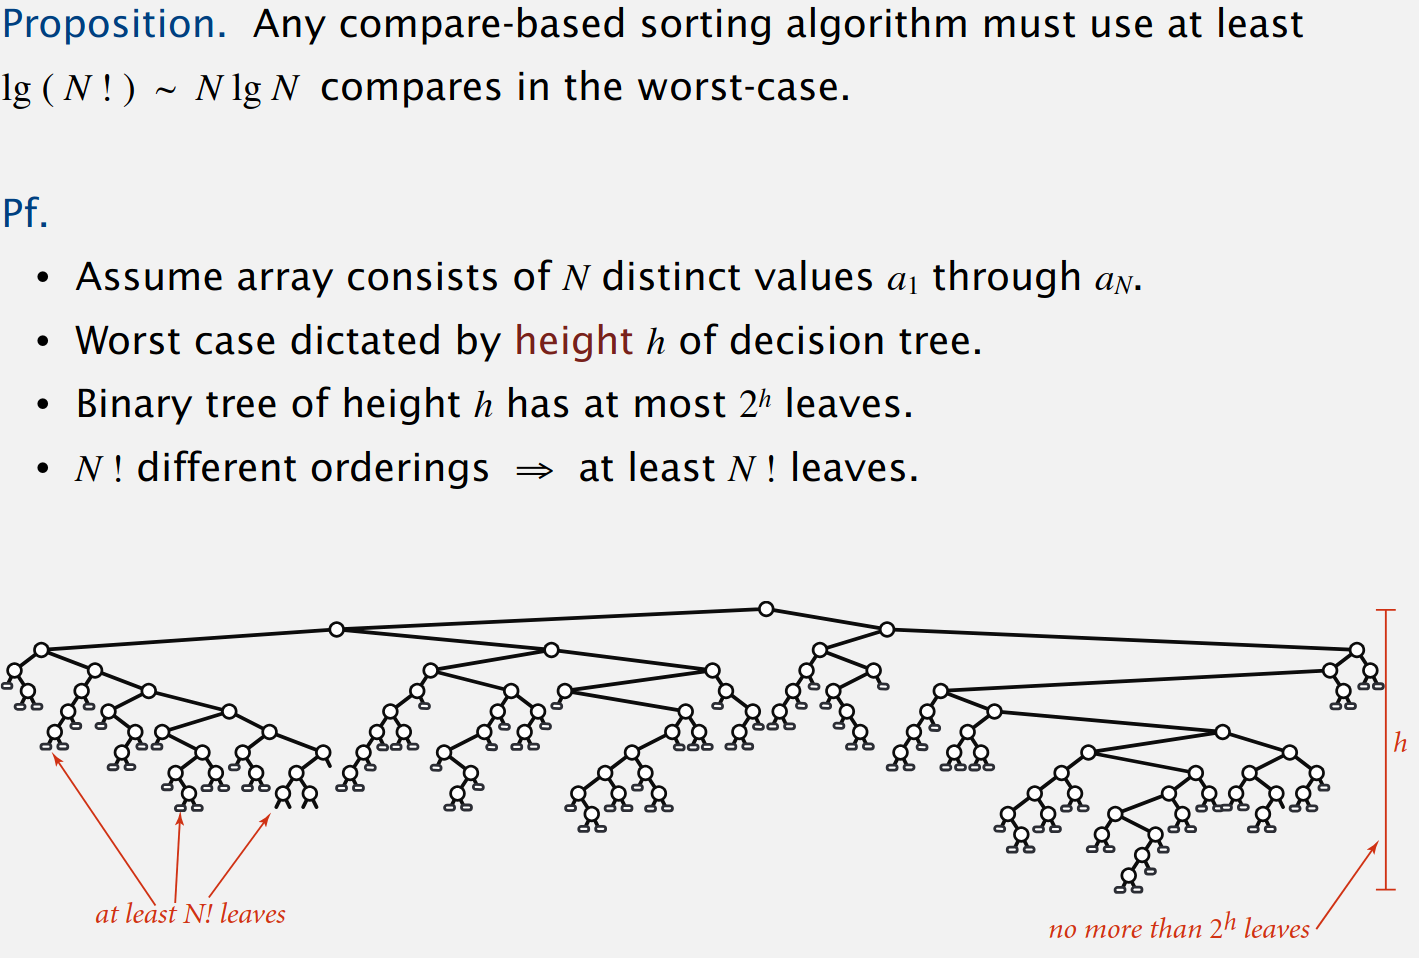
\includegraphics[width=110mm, height=65mm]{compare_based_tree_2}} 

\end{figure}
\end{frame}

%%%%%%%%%%%%%%%%%%%%%%%%%%%%%%%%%%%%%%%%%%%%%%%%%%%%%%%%%%%%%%%%%%%%%%%%%%%%%%%%%%%%%%%%%%%%%%%%%%
\begin{frame}
\frametitle{Дополнения}
\framesubtitle{Сортировки на сравнениях}
\justifying
\begin{figure}
    \captionsetup[subfigure]{labelformat=empty}
    \centering
    \subfigure[{ \scriptsize  Идея доказательства, Источник - \href{https://algs4.cs.princeton.edu/lectures/keynote/22Mergesort.pdf}{Alg4cs Princeton - Sedgewick \& Wayne}}]{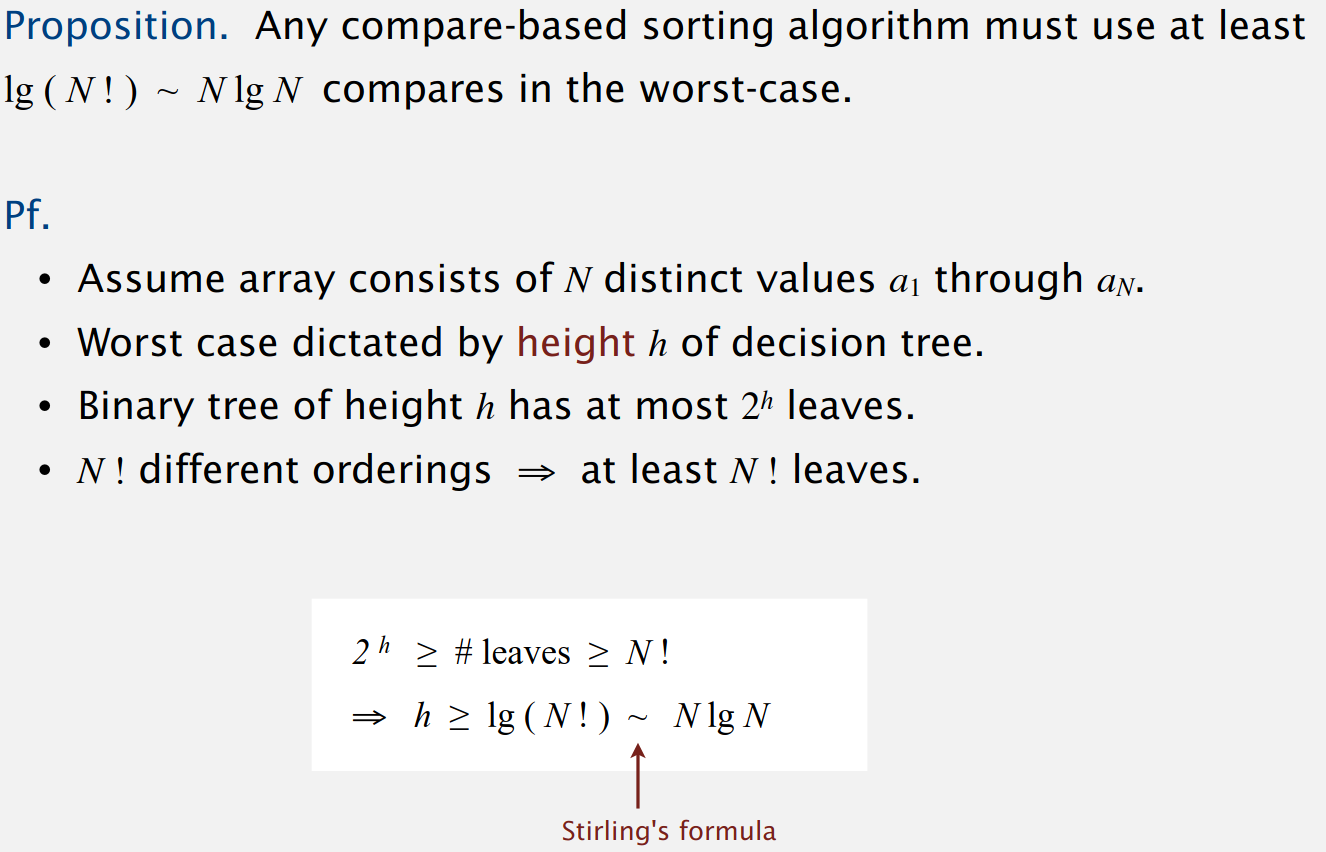
\includegraphics[width=110mm, height=65mm]{compare_based_proof}} 

\end{figure}
\end{frame}

%%%%%%%%%%%%%%%%%%%%%%%%%%%%%%%%%%%%%%%%%%%%%%%%%%%%%%%%%%%%%%%%%%%%%%%%%%%%%%%%%%%%%%%%%%%%%%%%%%
\begin{frame}
\frametitle{Дополнения}
\framesubtitle{Стабильность}
\justifying
\begin{figure}
    \captionsetup[subfigure]{labelformat=empty}
    \centering
    \subfigure[{ \scriptsize  Стабильность сортировки - Пример, Источник - \href{https://algs4.cs.princeton.edu/lectures/keynote/22Mergesort.pdf}{Alg4cs Princeton - Sedgewick \& Wayne}}]{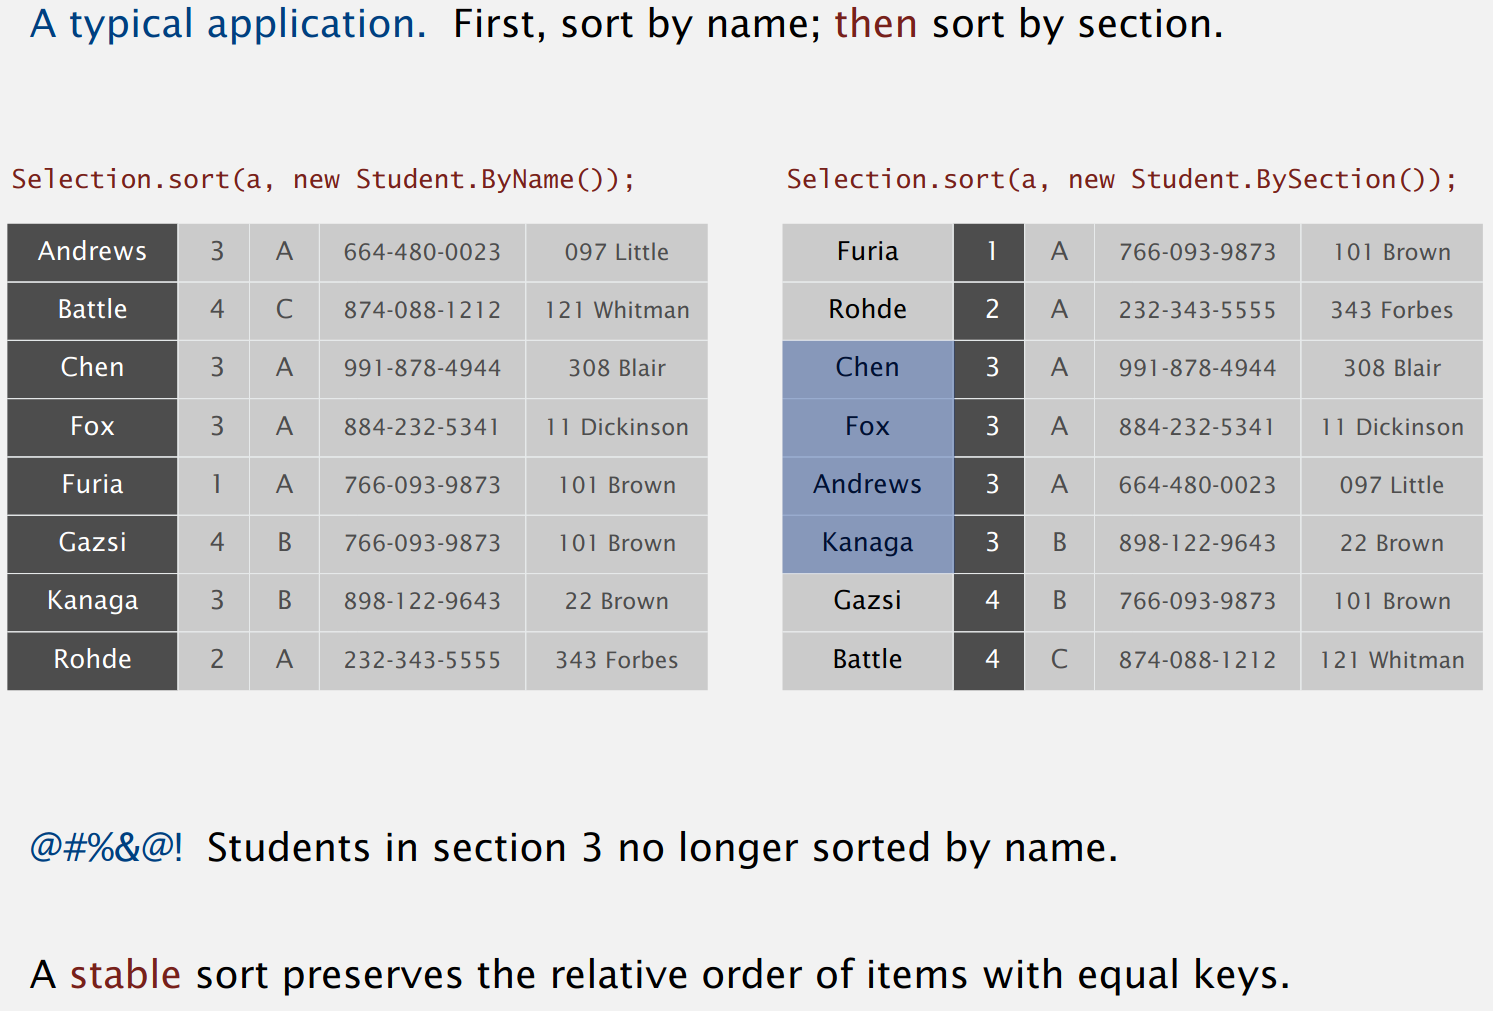
\includegraphics[width=110mm, height=65mm]{stability_example}} 

\end{figure}
\end{frame}

%%%%%%%%%%%%%%%%%%%%%%%%%%%%%%%%%%%%%%%%%%%%%%%%%%%%%%%%%%%%%%%%%%%%%%%%%%%%%%%%%%%%%%%%%%%%%%%%%%
\begin{frame}
\frametitle{Дополнения}
\framesubtitle{Стабильность - сортировка вставками}
\justifying
\begin{figure}
    \captionsetup[subfigure]{labelformat=empty}
    \centering
    \subfigure[{ \scriptsize  Стабильность, вставки - Пример, Источник - \href{https://algs4.cs.princeton.edu/lectures/keynote/22Mergesort.pdf}{Alg4cs Princeton - Sedgewick \& Wayne}}]{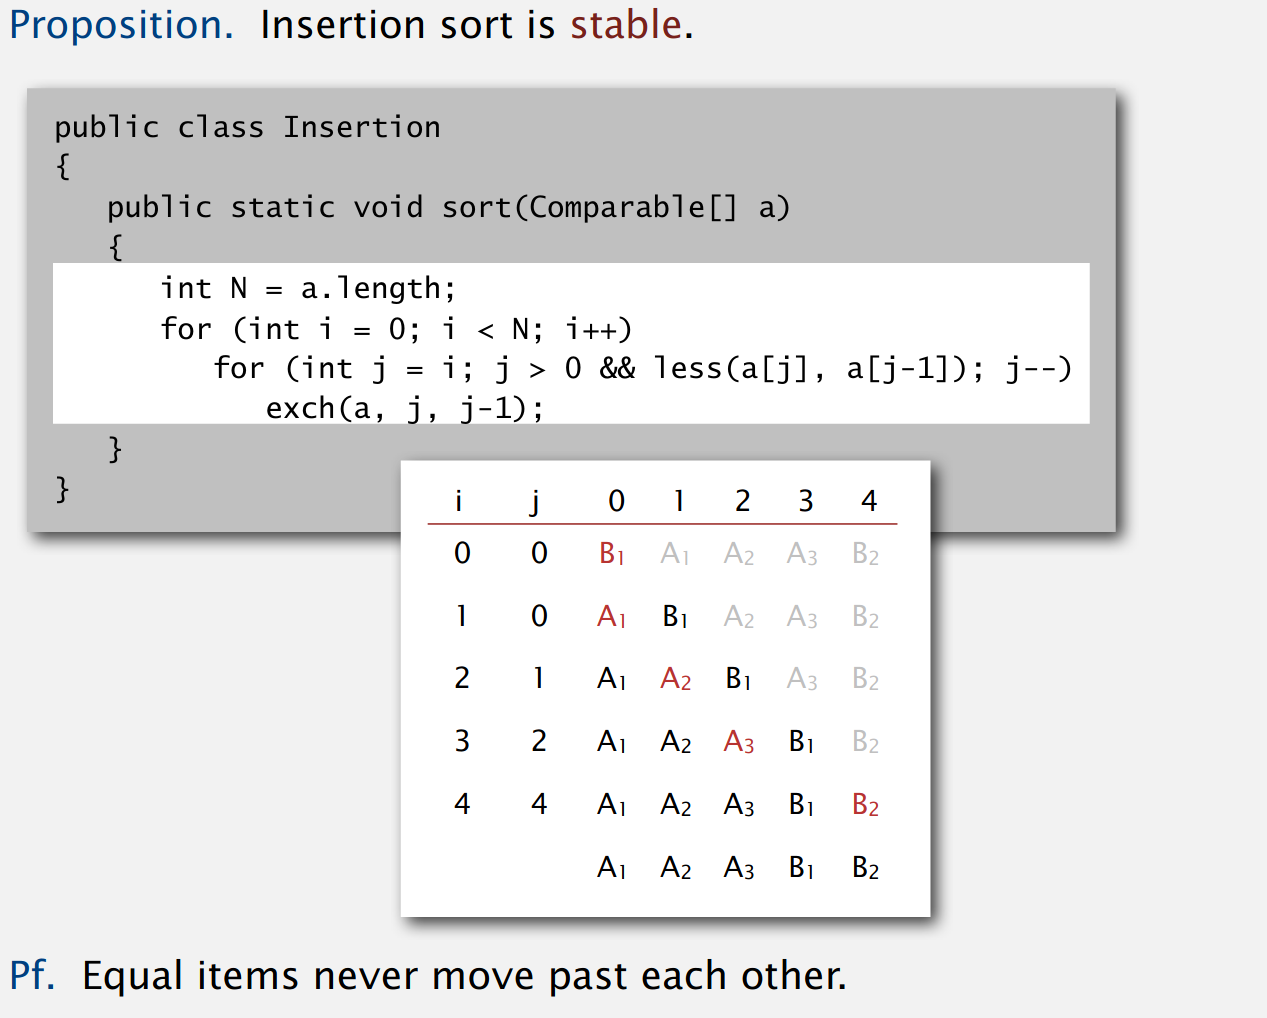
\includegraphics[width=100mm, height=65mm]{stability_insertion}} 

\end{figure}
\end{frame}

%%%%%%%%%%%%%%%%%%%%%%%%%%%%%%%%%%%%%%%%%%%%%%%%%%%%%%%%%%%%%%%%%%%%%%%%%%%%%%%%%%%%%%%%%%%%%%%%%%
\begin{frame}
\frametitle{Дополнения}
\framesubtitle{Стабильность - сортировка выбором}
\justifying
\begin{figure}
    \captionsetup[subfigure]{labelformat=empty}
    \centering
    \subfigure[{ \scriptsize  Стабильность, выбор - Пример, Источник - \href{https://algs4.cs.princeton.edu/lectures/keynote/22Mergesort.pdf}{Alg4cs Princeton - Sedgewick \& Wayne}}]{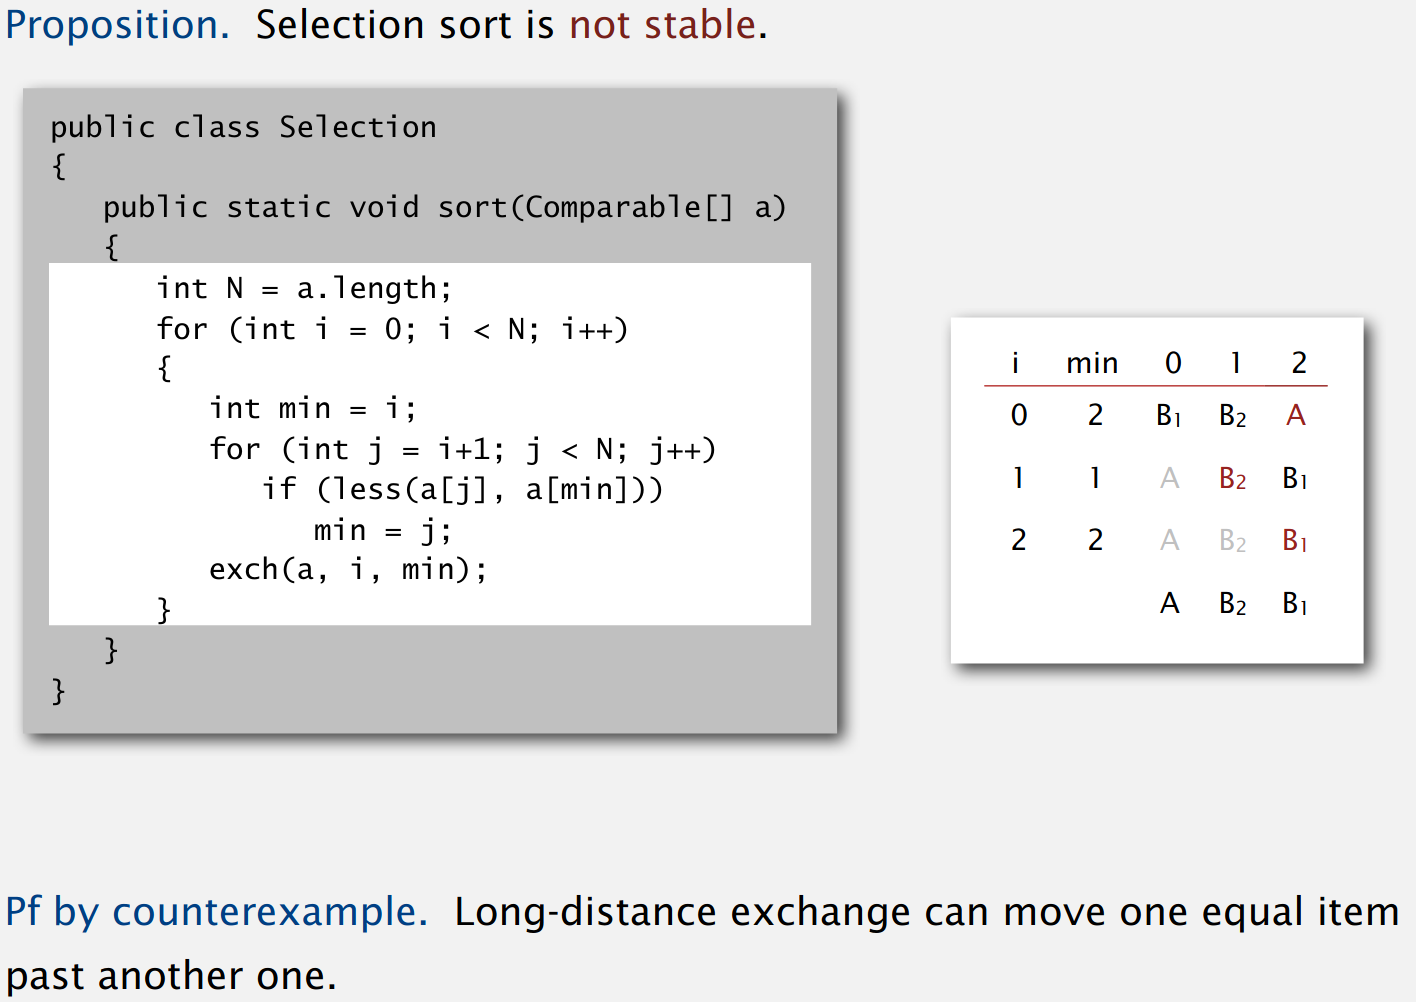
\includegraphics[width=100mm, height=65mm]{stability_selection}} 

\end{figure}
\end{frame}

%%%%%%%%%%%%%%%%%%%%%%%%%%%%%%%%%%%%%%%%%%%%%%%%%%%%%%%%%%%%%%%%%%%%%%%%%%%%%%%%%%%%%%%%%%%%%%%%%%
\begin{frame}
\frametitle{Дополнения}
\framesubtitle{Стабильность - слияние}
\justifying
\begin{figure}
    \captionsetup[subfigure]{labelformat=empty}
    \centering
    \subfigure[{ \scriptsize  Стабильность, слияние - Пример, Источник - \href{https://algs4.cs.princeton.edu/lectures/keynote/22Mergesort.pdf}{Alg4cs Princeton - Sedgewick \& Wayne}}]{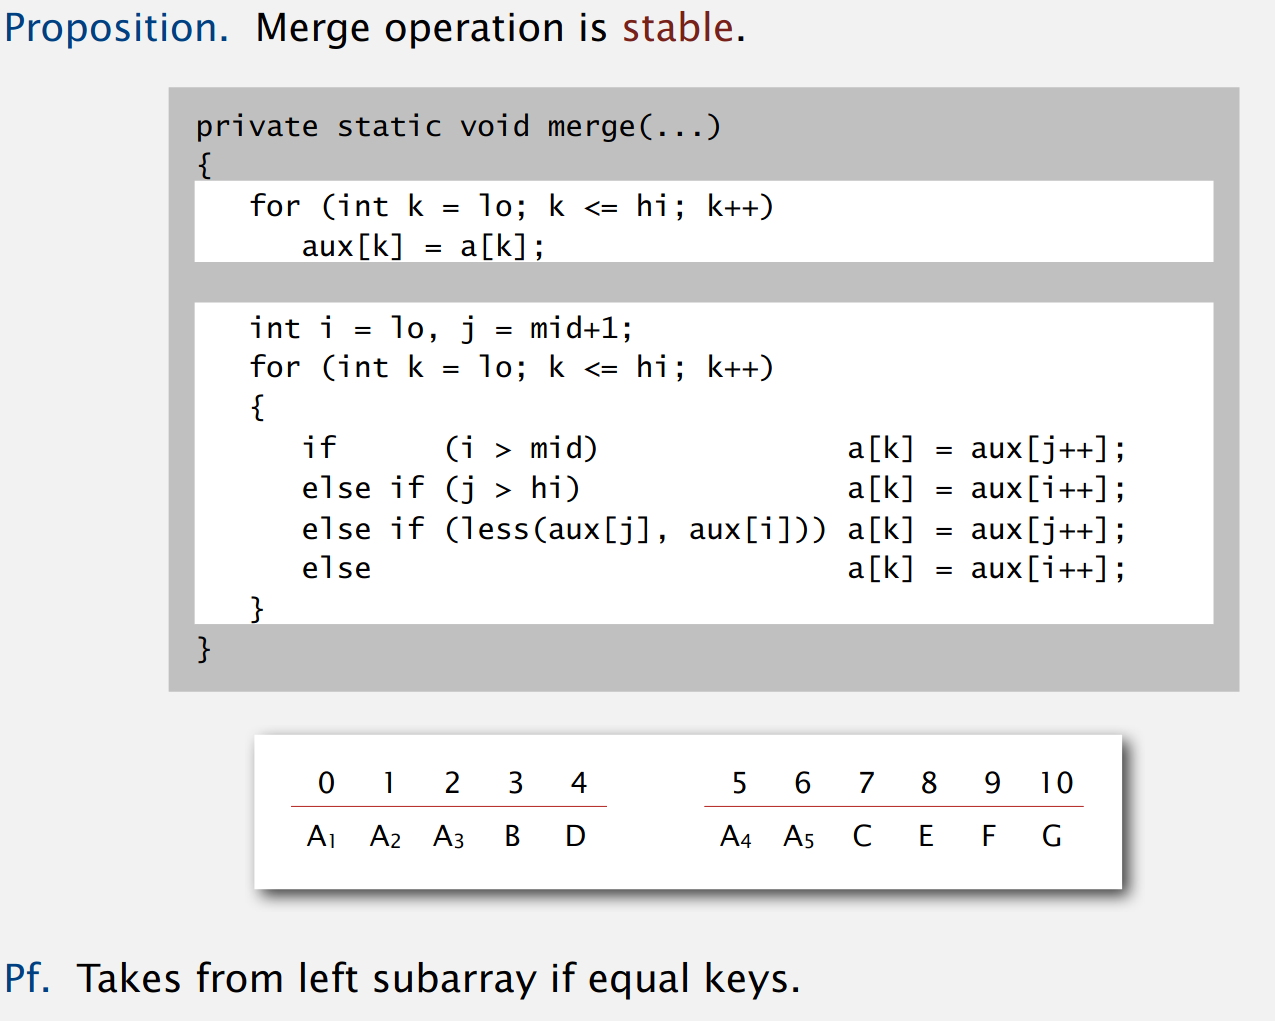
\includegraphics[width=100mm, height=65mm]{stability_merge}} 

\end{figure}
\end{frame}


%%%%%%%%%%%%%%%%%%%%%%%%%%%%%%%%%%%%%%%%%%%%%%%%%%%%%%%%%%%%%%%%%%%%%%%%%%%%%%%%%%%%%%%%%%%%%%%%%%
\begin{frame}
\frametitle{Дополнения}
\framesubtitle{Стабильность - быстрая сортировка}
\justifying
\begin{figure}
    \captionsetup[subfigure]{labelformat=empty}
    \centering
    \subfigure[{ \scriptsize  Стабильность, быстрая - Пример, Источник - \href{https://algs4.cs.princeton.edu/lectures/keynote/22Mergesort.pdf}{Alg4cs Princeton - Sedgewick \& Wayne}}]{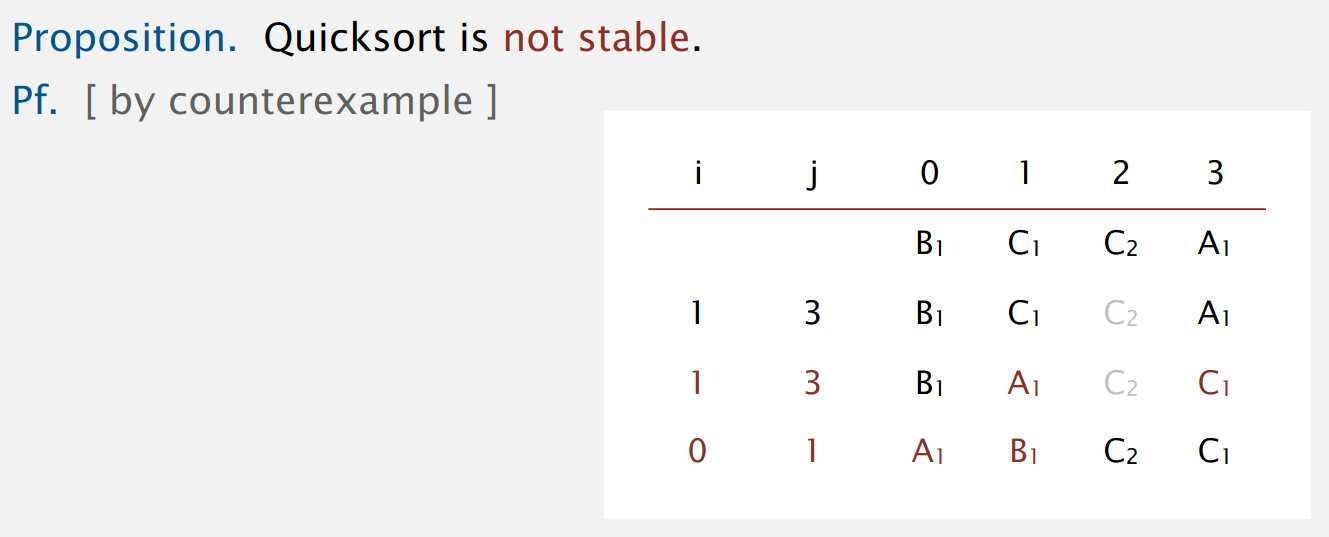
\includegraphics[width=100mm, height=40mm]{stability_qs}} 

\end{figure}
\end{frame}

%%%%%%%%%%%%%%%%%%%%%%%%%%%%%%%%%%%%%%%%%%%%%%%%%%%%%%%%%%%%%%%%%%%%%%%%%%%%%%%%%%%%%%%%%%%%%%%%%%
\begin{frame}
\frametitle{Дополнения}
\framesubtitle{Сложность сортировок}
\justifying
\begin{figure}
    \captionsetup[subfigure]{labelformat=empty}
    \centering
    \subfigure[{ \scriptsize  Сортировки, Источник - \href{https://algs4.cs.princeton.edu/lectures/keynote/22Mergesort.pdf}{Alg4cs Princeton - Sedgewick \& Wayne}}]{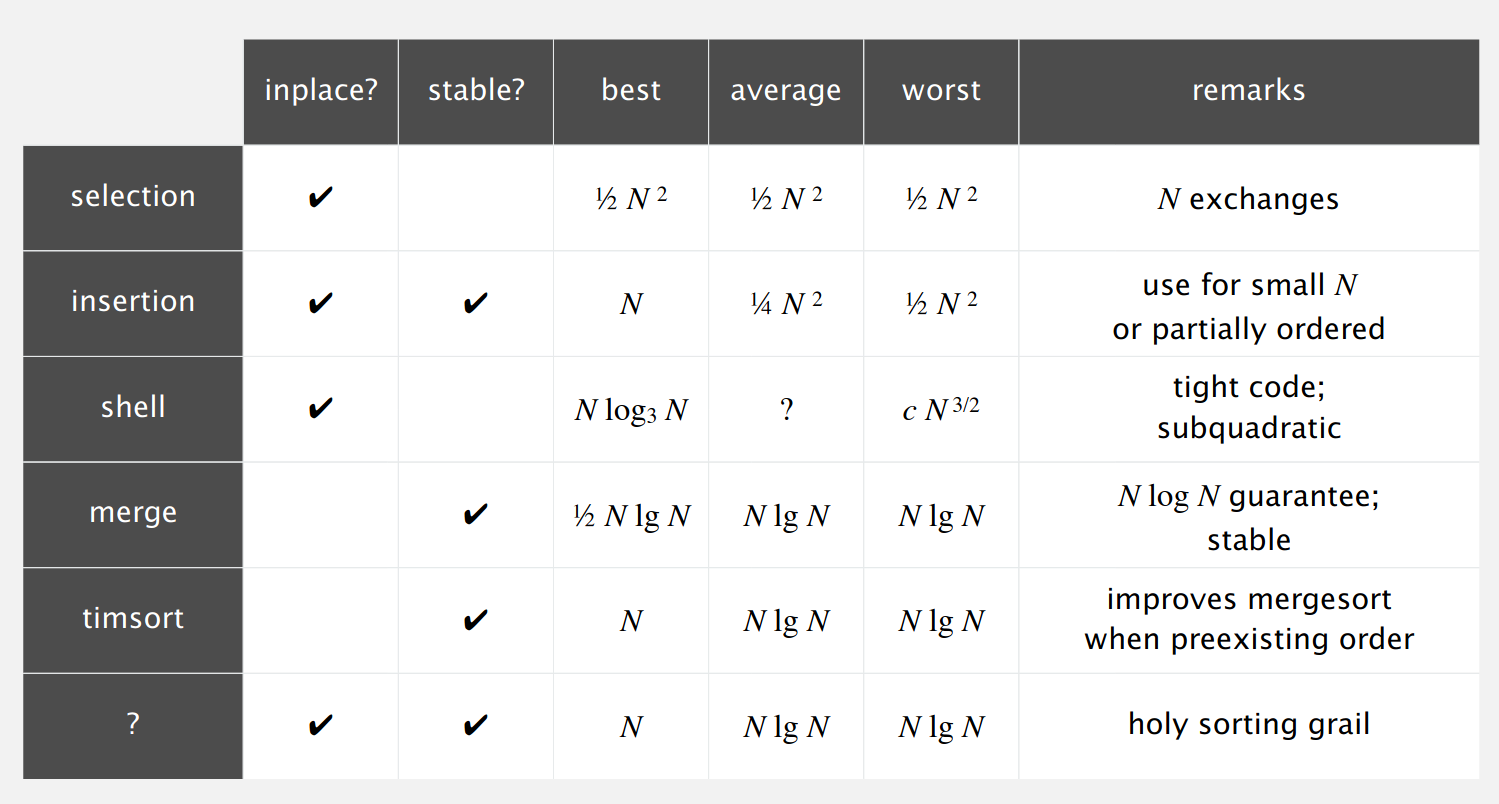
\includegraphics[width=120mm, height=60mm]{summary_sedgewick}} 

\end{figure}
\end{frame}

%%%%%%%%%%%%%%%%%%%%%%%%%%%%%%%%%%%%%%%%%%%%%%%%%%%%%%%%%%%%%%%%%%%%%%%%%%%%%%%%%%%%%%%%%%%%%%%%%%
\begin{frame}
\frametitle{Дополнения}
\framesubtitle{Сложность сортировок}
\justifying
\begin{figure}
    \captionsetup[subfigure]{labelformat=empty}
    \centering
    \subfigure[{ \scriptsize  Сортировки, Источник - \href{https://algs4.cs.princeton.edu/lectures/keynote/22Mergesort.pdf}{Alg4cs Princeton - Sedgewick \& Wayne}}]{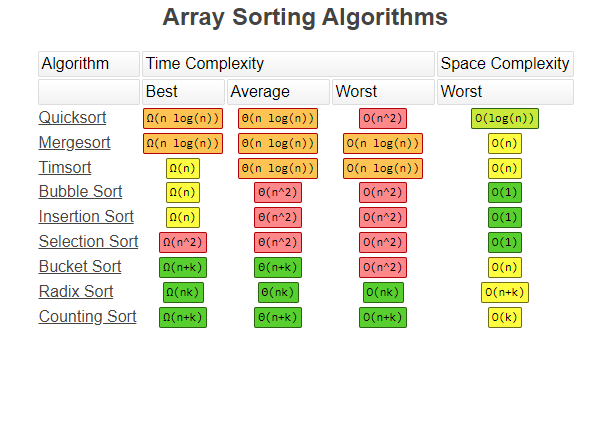
\includegraphics[width=120mm, height=80mm]{summary_all}} 

\end{figure}
\end{frame}



\end{document}